The angle of elevation is essential to calculate the geometry of our constellation. As discussed previously, our aim in this project report is to justify how global coverage will be fulfilled. First, it must be defined as the elevation angle for a given groundstation as the angle between its beam pointing right to the satellite and the horizontal local plane. Secondly, a study is conducted in order to relate the height of the satellite, the elevation angle and the coverage of the Earth. Finally, the orbital design is completed by configuring a constellation that will securely define a global coverage fulfillment. Below, these parameters will be defined and related. 

\begin{figure}[h]
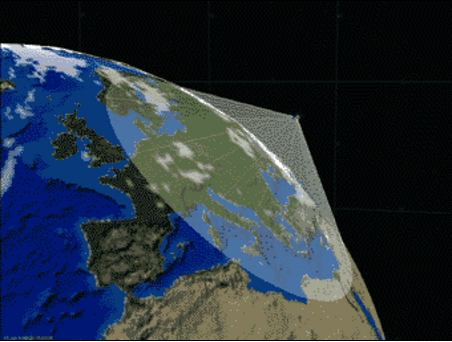
\includegraphics[width=8cm]{noaa}
\centering
\caption[Elevation angle cone]{Elevation angle cone. Source: NOAA}
\end{figure}

\subsection{Elevation angle cone}

Global coverage will be discussed considering the elevation angle and its resulting footprint on Earth. The elevation angle is described by the angular orientation of the antennas in the ground station. However, this angle is also perceived by the satellite in a similar way - it will vary depending on the orientation of the satellite and the angle between horizontal local planes. In order to describe the footprints a cone must defined which vertex is set at the antennas of the satellite, pointing down to Earth, and which generatrix is given by the angle of elevation. This elevation angle based cone is the description of the paths that our communications can take place. In other words, the generatrix of this cone is setting the limits in which the antenna will operate as function of the elevation angle. This implies that our satellite will be able to communicate to all the points contained in the cone. Finally, this cone will be describing a circular surface on top of the Earth which will be called the footprint of the satellite. Additionally, this footprint is the coverage that a single satellite can generate, hence the satellites will be distributed all around the Earth in order to fulfill global coverage. 

\subsection{Atmospheric restrictive conditions}
In order to obtain the final restrictive angle of elevation needed to contact the ground stations some considerations have to be made. Then, the bandwidth will be studied in order to analyse if they must be taken into account when communicating with ground stations \cite{Gomez2013}. The most important parameters are the following:

\begin{itemize}
\item\textbf{ Atmospheric gases: }water vapour and oxygen absorptions; important when frequencies are above 3 GHz. More information \cite{Zubair2011} and \cite{Luini2015}.
\item\textbf{ Precipitations and Clouds: }these conditions are relevant for signals above 10GHz.
\end{itemize}

By means of these physical phenomena we can substract the elevation angle as function of the latitude. However, we must take into account that these physical conditions give a value for the elevation angle which may not be the most restrictive. Global coverage conditions, bandwidths, inclination and the final distribution of our constellation will be considering this elevation angle and viceversa, iteratively.

The ASTREA CONSTELLATION was designed and optimized in order to fulfill global coverage for a constant elevation angle - respect to the latitude - of 20 degrees. This corresponds to a predefined model.

Analysing the minimum elevation angle needed in order to fulfill global coverage requieres, as mentioned before, the understanding first of the restrictive conditions of the atmosphere and how these will alter it. As a consequence of the different physical conditions given before we will be able to determine a relation between latitude and elevation angle. All the same, the elevation angle depends on the bandwith in which the satellites operate, hence different distributions of this angle respect to the latitude will be described depending on the bandwidths used. 

Our constellation will be operating at S-band for telemetry and X-band for data relay. Therefore, the satellites need to be operating up to 10 GHz. This directly implies that physical conditions such as atmospheric gases, precipitations and clouds must be studied when determining the elevation angle needed. We can obtain a more realistic model for the elevation angle comparing the frequencies of our constellation to others that are currently operative. Taking into account these considerations, this realistic model will have a peak at around 70 degrees in terms of elevation angle needed which will have a value near 30 degrees. This is due to the inclination of the orbit described (72 degrees). The value of the elevation angle, as discussed in \cite{Li2016} depends basically on the frequencies at which the antennas of our satellites work. The fact that the signals are X-band based means that the antennas will work with frequencies of 10 GHz as mentioned before, which means that the the atmospheric gases will be atenuating the signal in a significant way as the satellite is transmitting data with frequency higher than 3 GHz. Some further conclusions:

\textendash\  At low latitudes (between 0 and 30 degrees) the constellation fulfills global coverage generously.

\textendash\ At ground station latitude (60 degrees) the constellation is covering the station succesfully. For the previous model (constant elevation) coverage was well established with margin - as we set global coverage from the equator. For the latter model, this is the latitude at which the elevation angle corresponds to that defined constant in the first model, ergo works analogously. Note: each orbit could be reduced to a lower number of satellites per plane, but this would endanger the correct and stationary behaviour of the constellation. In fact, in this case we would not be able to control possible incidencies such as unoperative satellites with enough margin.

\textendash\ The ground stations are covered at all time for at least one satellite.

\subsection{Elevation angle of other current constellations}
\textendash\ Celestri: 18.8 to 20.2 GHz at 48 degree inclination.

\textendash\ GlobalStar: 2.4 GHz at 52 degree inclination.

\textendash\ Iridium: 20 to 30 GHz at 90 degree inclination - polar orbits.

Comparing our configuration to other present constellations some clarifications can be made: 

\textendash\ The minimum elevation angle peak is proportional to the bandwidth at which the satellite is communicating with Earth. For instance, Iridium's peak of elevation angle is the highest relative to the other configurations since it is also working with the highest frequency signals.

\textendash\ The latitude position of the peaks is related to the inclination of the constellation. Iridium, - a polar orbit based configuration - describes a peak at 90 degrees of latitude whereas Celestri and GlobalStar are near 40 to 50 degrees.

With these tendencies our model can be likewise described. This model would be defined by a peak at about 70 degrees latitude, smaller than those of the Celestri and Iridium constellations, but higher compared to the Iridium constellation peak. Thus, the previous model of a constant 20 degree elevation angle fulfills these requirements. 

\begin{figure}[h]
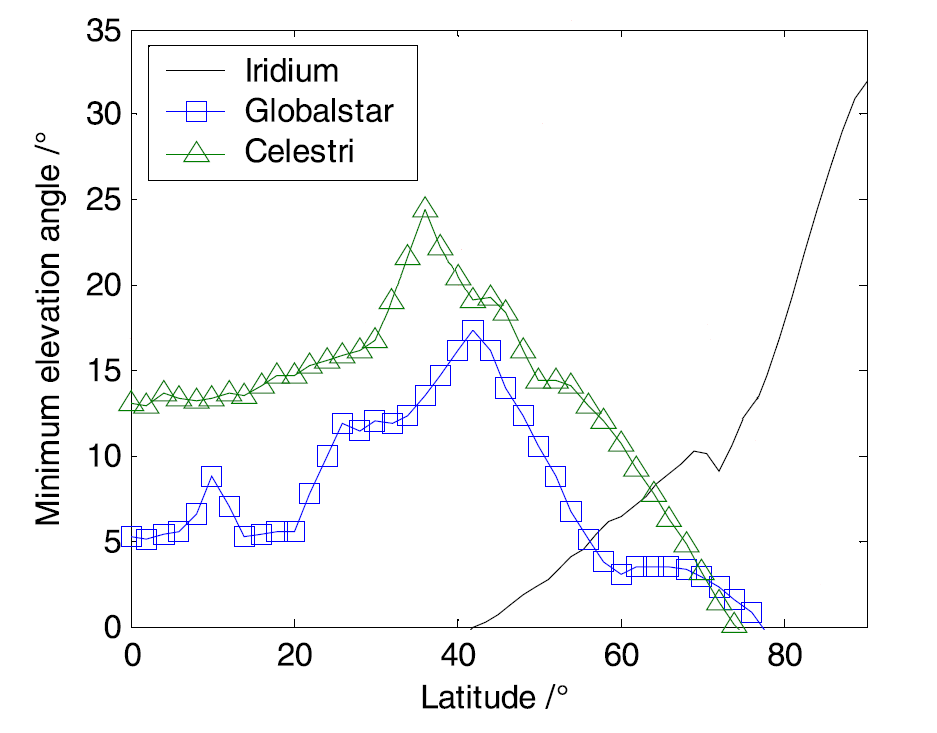
\includegraphics[width=8cm]{latitudes}
\centering
\caption[Minimum elevation angle as function of latitude]{Minimum elevation angle as function of latitude. Source: \cite{Li2016}}
\end{figure}